\section{Excurse}
\subsection{Gradient Descent}
\subsubsection{Optimization Using Gradient Descent}
We now consider the problem of solving for the \textit{minimum} of a real-values function
\begin{align}
	\min_{x} f(x).
\end{align}
We assume
\begin{itemize}
	\item $f:\R^4 \rightarrow R$ captures the machine learning problem at hand,
	\item $f$ is differentiable,
	\item we are unable to analytically find the solution in closed form.
\end{itemize}
The \textit{gradient descent} takes steps a proportionaly ($\gamma$) to the negative of the gradient of the function $\nabla f$ at the current point $x_0$:
\begin{align}
	\nabla x_1 = x_0 - \gamma ((\nabla f)(x_0))^T.
\end{align}
At the point $x_0$ the function $f(x_0)$ degresses fastes if on moves from $x_0$ in the direction of the negative gradient $- \gamma ((\nabla f)(x_0))^T$ of $f$ at $x_0$. From this follows: For a small \textit{step-size}\footnote{In Azure ML is called \textit{learning-rate}} $\gamma \geq 0$ $f(x_1)\geq f(x_0)$.\\

\paragraph{The Simple Gradient Descent Algorithm}
To find the \underline{local} optimum $f_{x_*}$ we start with a inial guess $x_0$ of the parameter we wish to optimize. Then we iterate according to 

\begin{align}
	\nabla x_{i+1} = x_i - \gamma_i ((\nabla f)(x_i))^T.
\end{align}
For a suitable step-size $\gamma_i$, the sequence $f(x_0)\leq f(x_1) \leq ... $ converges to a \textit{local} minimum.

\paragraph{Graphical Gradient Descent}
Only if the step-size $\gamma$ is a big, that the $f(x_{i+1}$ overshots the local minimum, the functional value $y=f(x_{i})$ converges to the local minimum.

\begin{figure}[H]
	\centering
	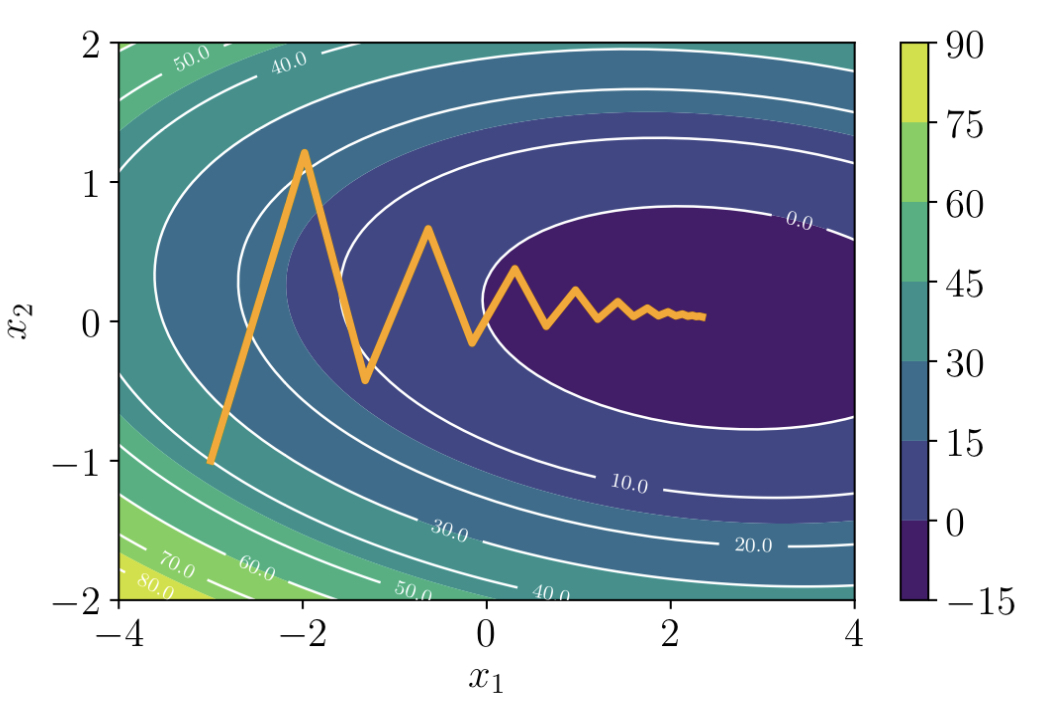
\includegraphics[scale = 0.2]{attachment/chapter_10/Scc053}
	\caption{Graph shows the gradient descent on a two dimensional quadratic surface.}
\end{figure}


The zig-zag of the graph

\begin{figure}[H]
	\centering
	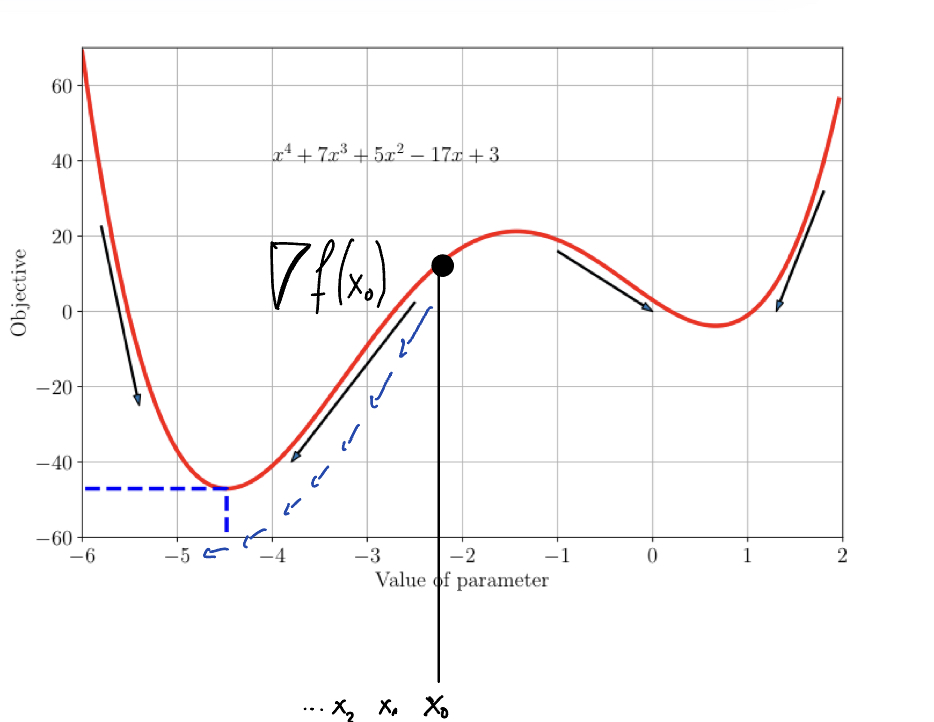
\includegraphics[scale = 0.2]{attachment/chapter_10/Scc052}
	\caption{Example of a one dimentional function. Negative gradient descent is indicated by the arrows.}
\end{figure}

\subsubsection{Solving a Linear Equation System}
\paragraph{In Form Ax=b}

